\chapter{The role of convex functions in the optimisation}

In this lecture we take a close look at the role of convex functions in the optimization problems. 

First we review some key definitions from the previous Proseminars. Afterwards, we take a look at some examples and lastly, we define theorems which we are going to use as a base for explaining the correlation between the convexity of functions and the optimisation problems.


We begin this topic with revision of some of the key terms defined in the previous lectures of this Proseminar.

\begin{definition}[Convex set]
	A set $X \subseteq \R^n$  is a \textbf{convex set}, if for all $x_1, x_2\in X$ and all $\lambda\in(0,1)$ it holds: 
	\begin{align}
	\lambda x_1 + (1-\lambda) x_2\in X \label{definition:1:convexset} %\tag{1}
	\end{align}
	% you dont need the \tag{...} if you use align instead of align*
	% usually the * prevents numbering, also in chapter or section commands
\end{definition} 

\begin{definition}[Convex, strictly and uniformly convex function:]
	Let $X\subseteq\R^n$ be a convex set. A function $f:\R^n\rightarrow\R$ is:
	\begin{enumerate}   
		\item \textbf{convex} on X, if for all $x_1, x_2 \in X$ and all $\lambda\in(0,1)$ holds: 
		\begin{align}
		f(\lambda x_1 + (1-\lambda) x_2) \le \lambda f(x_1)+(1-\lambda)f(x_2)
		\label{definition:2:convex} %\tag{2}
		\end{align}
		
		\item \textbf{strictly convex} on X, if for all \(x_1, x_2\in{X}\) and all \(\lambda\in(0,1)\) holds
		\begin{align}
		f(\lambda{x_1} + (1-\lambda){x_2}) < \lambda f(x_1)+(1-\lambda)f(x_2)
		\label{definition:3:strictlyconvex}
		\end{align}
		
		\item \textbf{uniformly convex} on X, if there exists $\mu > 0$ with:
		\begin{align}
		f(\lambda x_1 + (1-\lambda) x_2) + \mu\lambda (1-\lambda)\left\lVert x_1-x_2\right\rVert^2 \le \lambda f(x_1)+(1-\lambda)f(x_2)
		\label{definition:4:uniconvex}
		\end{align}
	\end{enumerate}  
\end{definition}

Now we begin with defining our first theorem:

\begin{satz}
	Let $f:\R^n\to\R$ be convex. Then, the level sets
	\begin{align*}
	\mathcal{L}(x_0) &:= \{ x\in\R^n | f(x)\leq f(x_0) \}  \\
	\mathcal{L}(x_0) &:= \{ x\in\R^n | f(x) < f(x_0) \}
	\end{align*}
	are for all $f(x_0)\in\R$, convex.
\end{satz}

\begin{proof}
	\begin{itemize}
		\item The objective of this proof is to show that the set $\mathcal{L}(x_0)$ is convex, that is, for all $x_1, x_2 \in \mathcal{L}(x_0), \lambda\in (0,1) : \lambda x_1 + (1-\lambda) x_2 \in\mathcal{L}(x_0)$.
		
		Let $x_1, x_2 \in X, \lambda\in (0,1)$. Looking at the preconditions of this theorem, we see that $f$ is convex, which according to inequality \labelcref{definition:2:convex} means:  % labelcref takes the number of label definition:2:convex which is related to equation 2 above
		\begin{align*}
		f ( \lambda x_1 + (1-\lambda) x_2 ) \leq \lambda f(x_1) + (1-\lambda)f(x_2)
		%\text{ for } x_1, x_2 \in X, \lambda\in (0,1). 
		\end{align*}
		Then for $x := \lambda x_1 + (1-\lambda) x_2$, it holds:
		\begin{align*}
		f(x) &= f(\lambda x_1 + (1-\lambda) x_2) \\
		&\overset{\labelcref{definition:2:convex}}{\leq} \lambda f(x_1) + (1-\lambda)f(x_2)\\
		&\overset{(*)}{\leq} \lambda f(x_0) + (1-\lambda) f(x_0)\\
		&= f(x_0)
		\end{align*}
		(2) it follows from the convexity of the function $f$ \\ 
		% i would say that you dont need this once more to say, beacause equation (2) already says this
		(*) since $x_1, x_2 \in \mathcal{L}(x_0)$, it follows that $f(x_1), f(x_2) \leq f(x_0)$
		% i would state (*) before the equation
		%
		\item The proof that the level set $\mathcal{L}(x_0) := \{ x \in \R^n | f(x) < f(x_0) \}$ is for all $f(x_0) \in \R$, convex, follows analogously with the use of the proof of the first part with ("$<$") instead of ("$\leq$"). 
	\end{itemize}
\end{proof}

Next, we go back to the optimisation problems and explain why the class of (strict, uniform) convex functions play an important role in the optimisation. 
\begin{satz} \label{theorem:4}
	Let $f:X\rightarrow\R$ be continuously differentiable and $X\subseteq\R^n$ be convex with $x\in X$. We consider the restricted optimization problem
	\begin{align}
	\min (f(x))  \label{theorem:5:opt}
	\end{align}	
	Then the following statements hold:
	\begin{enumerate}
		\item If the function $f$ is \textbf{convex} on $X$, then the solution set of \labelcref{theorem:5:opt} is \textbf{convex (or empty)}
		\item If the function $f$ is \textbf{strictly convex} on $X$, then the solution set of \labelcref{theorem:5:opt} has \textbf{at most one solution} 
		\item If the function $f$ is \textbf{uniformly convex} on $X$, $X \neq \emptyset$ and $X$ is a closed set, then \labelcref{theorem:5:opt} has \textbf{exactly one solution}
		\begin{enumerate}
			\item If the function $f$ is \textbf{uniformly convex} on $X$ but $X$ is not empty, then \labelcref{theorem:5:opt} has no solution
			\item If the function $f$ is \textbf{uniformly convex} on $X$ but $X$ is not a closed set, then \labelcref{theorem:5:opt} has no solution.
		\end{enumerate}\subitem 
	\end{enumerate}
\end{satz}

\begin{proof}
	\begin{enumerate}[label=(\arabic*)]
		\item Objective: to show that for $x_1, x_2 \in \min f(x)$ and $\lambda \in (0,1)$ , it holds: $\lambda x_1+(1-\lambda)x_2 \in \min(f(x)).$ 
		
		Let $x_1, x_2 \in min(f(x))$  (which means that $x_1$ and $x_2$ are two solutions of \labelcref{theorem:5:opt}, that is, $f(x_1)=f(x_2)=min(f(x))$. From the convexity of $X$, it holds: $\lambda x_1 +(1-\lambda) x_2 \in X$, for $\lambda\in (0,1)$. Therefore, from the convexity of $f$ it follows: 
		\begin{align*}
		f(\lambda x_1+(1-\lambda)x_2) &\overset{\labelcref{definition:2:convex}}{\leq}\lambda f(x_1)+(1-\lambda)f(x_2)\\
		&= \lambda f(x_1)+f(x_2)-\lambda f(x_2)  \quad \text{because } f(x_1)=f(x_2)\\
		&= \lambda f(x_1)+f(x_1)-\lambda f(x_1)\\
		&= f(x_1)\\
		&= \min(f(x))
		\end{align*}
		from where it follows that $f(\lambda{x_1}+(1-\lambda)x_2)\leq \min f(x)$ (minimum of the function $f$ and therefore $\lambda x_1 + (1-\lambda)x_2$ is a minimum of (1): $\lambda x_1 + (1-\lambda)x_2\in \min(f(x))$.
		
		\item We prove this next part of the Theorem through contradiction. \\ 
		Let the optimization problem \labelcref{theorem:5:opt} have two different solutions: $x_1$ and $x_2$ with $x_1 \neq x_2$ and $f(x_1)=f(x_2)=\min(f(x))$. Since $X$ is a convex set, for $\lambda\in (0,1)$ is $\lambda x_1 + (1-\lambda) x_2 \in X$. From the strict convexity of the function $f$ it holds that 
		\begin{align*}
		f( \lambda x_1 + (1-\lambda) x_2 ) &\overset{\labelcref{definition:3:strictlyconvex}}{<} \lambda f(x_1) + (1-\lambda) f(x_2)\\
		&\overset{(*)}{=}\lambda f(x_1) + f(x_1) - \lambda f(x_1)\\
		&= f(x_1) = \min(f(x)).
		\end{align*}
		where (*) follows from the fact that $f(x_1)=f(x_2)$. \\
		Therefore, we found an element of the set $X$, which is strictly smaller than all elements in the set $\min(f(x))$, which is in contradiction to the assumed minimality of $f(x_1)$.
		%
		\item Let $x_0\in X$ be arbitrarily selected. From Lemma 3.9 it follows that the level set $\mathcal{L}(x_0)$ is compact. So the set $X \cap \mathcal{L}(x_0)$ is also compact and, by definition, non empty. With the extreme value theorem, the continuous function $f$ has a global minimum on the compact set $X \cap \mathcal{L}(x_0)$, which from obvious reasons must also be a minimum of (1). 
		
		We now take a look just at the third part of the Theorem and ask ourselves, what would happen if the function $f$ was convex (and therefore strictly convex) and: 
		%we ask what would happen if f is uniformly convec, aren't we??
		\begin{enumerate}
			\item the set $X$ was empty: \\
			If $X$ was empty, then we would not have any points in $X \cap \mathcal{L}(x_0)$, which would trivially mean that the function $f$ would not have a minimum (as seen in \cref{example:5} (1))
			\item the set X was not closed. \\
			If $X$ was not closed, then the function $f$ would again trivially, not have a minimum (as seen in \cref{example:5} (2))
		\end{enumerate}
	\end{enumerate}
\end{proof}

Now we take a look at some counterexamples regarding \cref{theorem:4} (3): 

\begin{beispiel} \label{example:5}
	\begin{enumerate}[label=(\arabic*)]
		\item Let $f:\R\rightarrow\R$ with $f(x)=e^x$.
		\begin{proof} (The function \(f(x)=e^x\) is a convex function:) \\
			Since $\R$ is per definition a convex set, $f(x)=e^x$ is a continiously differentiable function as composition of continiously differentiable functions, and $\nabla{f(x)} = \nabla e^x = e^x$ is a monotone function, it follows that $f(x)=e^x$ is a convex function. \\
			Then, since the convex set $\R$ is not bounded, the function f(x)= $e^x$ is decreasing on the domain $\R$ for $x \rightarrow 0$ and never reaches a point of minimum, which means that the function does not have a minimum on the domain $\R$.
		\end{proof}
		\item Let $f:X\rightarrow\R$  with $X=\emptyset$. \\
		Then, since the convex set $X$ is empty, it does not contain any values $f(x)$, which trivially means that the function does not have a minimum.
	\end{enumerate}
	
	\begin{center}
		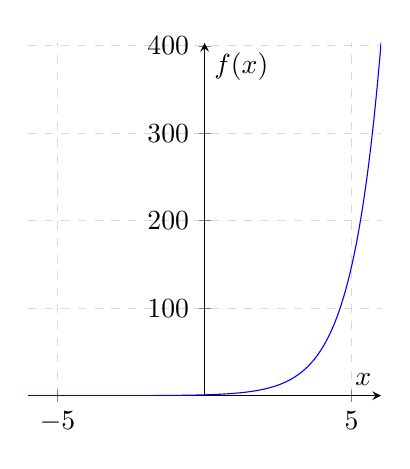
\begin{tikzpicture}
		\begin{axis}[
		samples=1000, 
		domain=-6:6,
		%	title=Niveaulinien von $F$,
		x label style={at={(axis description cs:1, 0)}, right},
		y label style={at={(axis description cs:0, 1)}, left, rotate=-90},
		xlabel=$x$,
		ylabel=$f(x)$,
		grid, 
		grid style={dashed,gray!30},
		axis y line=center,
		axis x line=center,
		xmin = -6,
		xmax = 6,
		width=0.5\textwidth,
		height=0.5\textwidth
		]
		\addplot[blue] {exp(x)};
		\end{axis}
		\end{tikzpicture}
	\end{center}
	% Here ends the furst plot
	
\end{beispiel}

We continue with defining an inequality for uniformly convex functions, which will be useful later on.

\begin{lemma}
	Let $f:\R^n\rightarrow\R$ be continuously differentiable, $x_0 \in\R^n$, the level set $\mathcal{L}(x_0)$ convex, $f$ uniformly convex on $\mathcal{L}(x_0)$ and $x \in\R$, according to Theorem 2, 3), unique global minimum of $f$. Then there exists $\mu>0$ with
	\begin{align*}
	\mu \left\lVert x-x^* \right\Vert^2 \leq f(x)-f(x^*) \qquad \forall \bigskip x \in \mathcal{L}(x_0)
	\end{align*}. 
\end{lemma}

\begin{proof}
	Using: 
	\begin{itemize}
		\item The inequality \labelcref{definition:3:strictlyconvex} from the begining of this lecture and 
		\item the fact that $x^*$ is, as a result of being a global Minimum of $f$, a stationary point of f and therefore $\nabla f(x^*)=0$,
	\end{itemize}
	we conclude the needed inequality.
\end{proof}

Finally, we analyze in which way the existence of stationary points of a function are connected to the existence of global minimum of that function.

\begin{satz}
	Let $f:\R^n\rightarrow\R$ be continuously differentiable and convex function, $x\in\R^n$ a stationary point of $f$. Then $x^*$ is a global minimum of $f$ on $\R^n$. 
\end{satz}

\begin{proof}
	First, we remind ourselves that a point $x^*\in X$ is called a stationary point of a continiously differentiable function $f:\R^n\rightarrow\R$, if $\nabla f(x^*)=0$.
	From Proposition 3.5. a) follows: 
	\begin{align*}
	f(x)-f(x^*)\leq\nabla f(x^*)^t (x^*)=0
	\end{align*}
	and thus 
	\begin{align*}
	f(x)\geq f(x^*), \forall x\in R
	\end{align*}
	It follows that $x^*$ is a global minimum of $f$.
\end{proof}